\subsubsection{Sinusträger, grobe Auflösung}
\label{6_2_2_title}
Bei diesem Verfahren wird die Netzspannung mit einem höher getakteten Dreiecksträger verglichen. Das Netz wird somit mehrmals abgetastet pro Periode. Diese Methode ist sehr einfach digital, wie auch analog zu implementieren.\\
\\

Falls $U_{Netz}$ grösser also $U_{Carrier}$ ist, wird $U_A$ auf $\frac{U_{dc}}{2}$ gestellt.

\begin{figure}[H]
  \begin{center}
  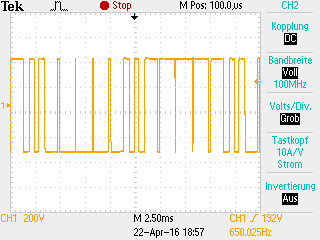
\includegraphics[width=0.48\textwidth]
  {pic/6_2_weitere_pulsmuster/6_2_1_stromform/carrier_grob/ALL0000/F0000TEK.png}
  \caption{$U_A (Orange)$}
  \label{fig:6_2_4_0}
  \end{center}
\end{figure}


\begin{figure}[H]
  \begin{center}
  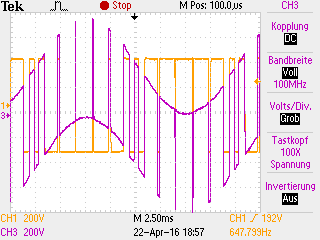
\includegraphics[width=0.48\textwidth]
  {pic/6_2_weitere_pulsmuster/6_2_1_stromform/carrier_grob/ALL0001/F0001TEK.png}
  \caption{$U_A (Orange), U_L (Violett)$}
  \label{fig:6_2_4_1}
  \end{center}
\end{figure}


\begin{figure}[H]
  \begin{center}
  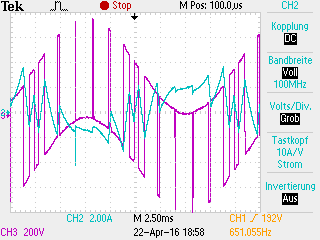
\includegraphics[width=0.48\textwidth]
  {pic/6_2_weitere_pulsmuster/6_2_1_stromform/carrier_grob/ALL0002/F0002TEK.png}
  \caption{$U_L (Violett), I_{L1} (Hellblau)$}
  \label{fig:6_2_4_2}
  \end{center}
\end{figure}
Dieses Pulsmuster enthält alle ungeraden Harmonischen. Je höher der Index der Harmonischen, desto kleiner die Energie.
Wirk und Blindleistung können weiterhin mit $\theta$ und $U_{dc}$ eingestellt werden.


\clearpage